% 第13章第5节：计算代价（状态表的规模、时间代价、存储代价、时间与存储的取舍）。

\section{计算代价}
\label{sec:graph-dp-computation-cost}

前几节的计算都给出精确结果，但所需的时间和存储可能很大。本节把已构建的袋和接口换算成实际的状态组合数，分别分析求值的时间、存储及二者的取舍。结构的构造方法见第~\ref{sec:graph-tree-decomposition-construction}节；这里给出的资源指标可以用来比较不同的构造结果，构造与核验本身的成本也一并计入任务的总成本。

\subsection{状态表的规模}
\label{sec:graph-dp-table-size}

先固定规模变量：变量个数$n$，局部项个数$|A|$，袋树节点数$N$，第$i$个变量的状态数$|\mathcal X_i|$，以及$q=\max_i|\mathcal X_i|$。对一组变量$U$，记它上面的配置数为
\[
|\mathcal X_U|=\prod_{i\in U}|\mathcal X_i| .
\]
计算中出现三类表：袋$u$上的合并表有$|\mathcal X_{B_u}|$项，接口消息和回溯表各有$|\mathcal X_{S_u}|$项（回溯表的每一项存$|I_u|$个变量的取值），保留变量的输出表有$|\mathcal X_R|$项。

在每个变量至多$q$个状态、分解宽度为$w$时，每个袋至多$w+1$个变量，袋表至多$q^{w+1}$项。但这只是上界：接口与输出仍按实际变量计算，状态数不同的变量对乘积的贡献也不同。比较两个候选结构时，应固定同一任务（同一保留集、同一输出要求），并使用实际的乘积，而不是只比较宽度。例如两个结构宽度都是$2$，一个的最大袋由三个二值变量组成（$8$项），另一个含一个十状态变量（至少$40$项），实际规模相差数倍。

图~\ref{fig:graph-dp-table-size}把这个差别落实为表项：两侧都只有三个变量，但十状态变量需要十组而不是两组配置。同为宽度$2$，并不意味着同样的读表和存储代价。

\begin{figure}[!htb]
  \centering
  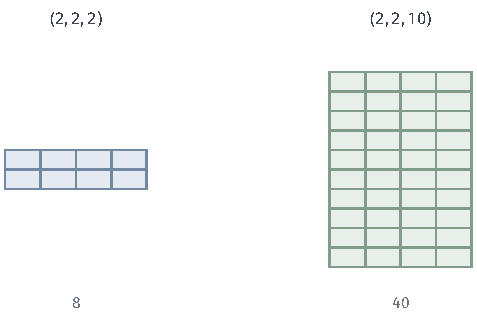
\includegraphics[width=80.617mm]{figures/03-graphs/04-local-functions-and-dynamic-programming/tikz/dp-table-size/figure.pdf}
  \caption{相同袋宽度下的实际表规模。括号给出三个变量各自的状态数，每格对应一种联合取值。左表为$2\times2\times2=8$项，右表为$2\times2\times10=40$项；四列枚举前两个二值变量，行枚举第三个变量。}
  \label{fig:graph-dp-table-size}
\end{figure}

宽度出现在指数上，这是精确计算的主要限制。$q=10$、$w=10$时一张袋表就有$10^{11}$项；若查询要求保留很多变量的联合表，输出本身也可能大得不可承受，这时任何精确方法都必须至少写出整张表。

四环算例中，分解$\{1,2,4\}-\{2,3,4\}$的两个袋各有$8$项，接口消息和回溯表各有$4$项；$R=\{1,3\}$的查询结构有两个$8$项的袋、一个$4$项的根袋，输出表$4$项。按次序$(1,2,3,4)$不合并时，四个消元簇的配置数为$8,8,4,2$。

\subsection{时间代价}
\label{sec:graph-dp-time-cost}

约定表查询、加法、乘法和比较各计一次基本运算。处理节点$u$时，要对$\bm x_{B_u}$的每种取值读取归入$u$的每个局部项一次、读取每条子消息一次，把它们组合起来，再参与一次取最小或求和，所以工作量约为
\[
|\mathcal X_{B_u}|\,\bigl(|A_u|+|\operatorname{ch}(u)|+1\bigr).
\]
对全部节点求和，利用袋树中$\sum_u|\operatorname{ch}(u)|=N-1$，求值时间为
\[
\sum_{u}|\mathcal X_{B_u}|\,\bigl(|A_u|+|\operatorname{ch}(u)|+1\bigr)=O\bigl((|A|+N)\,q^{w+1}\bigr).
\]
可见单个袋表的上界$q^{w+1}$还要乘以袋数和每项的工作量，才给出总时间。

按消元次序计算时，消去$x_i$要对$\{i\}\cup S_i$的至多$q^{|S_i|+1}$种取值各读取$\mathcal F_i$中每个函数一次，时间约为
\[
|\mathcal F_i|\,q^{|S_i|+1}.
\]
每个函数恰好在它的某个变量被消去时被取出一次，原有函数$|A|$个，新函数至多$n$个，所以各步的$|\mathcal F_i|$之和不超过$|A|+n$；按变量维护索引的开销也与函数个数成正比。若诱导宽度为$w$，总时间为
\[
O\bigl((|A|+n)\,q^{w+1}\bigr),
\]
而枚举为$|A|\,q^n$。

除向上的求值外，还要计入结果输出与配置恢复。条件最小成本表或累计表的输出要写出$|\mathcal X_R|$项。恢复一个配置时每个节点只查一次回溯表，共$O\bigl(\sum_u|B_u|\bigr)$次读写，与求值相比可以忽略。若还需要每个袋上各取值的最小总成本，就像第~\ref{sec:graph-dp-tree-two-pass}小节那样再按前序发送一遍反向消息，时间约加倍。

结构构造与核验的时间单独计算，再加入任务的总时间：模拟消元为$O\bigl(n+m+\sum_t d_t^2\bigr)$（第~\ref{sec:graph-dp-clusters-to-decomposition}小节），检验为袋大小的多项式（第~\ref{sec:graph-dp-construction-check}小节）。同一结构用于多组数值时，这部分只付一次。

计数中的整数加乘在上面各计一次基本运算。若要考虑位复杂度，还须按数值的位数分析：可行配置数至多为$\prod_i|\mathcal X_i|\leq q^n$，需要约$n\log_2q$位，大规模问题中一次加乘的实际代价随位数增长；加权求和若用浮点数，还要另行分析舍入误差。

\subsection{存储代价}
\label{sec:graph-dp-memory-cost}

存储要分清对象，并按计算过程中同时保留的对象计算峰值，不能把累计生成的表项总量或单个接口的规模直接当作峰值。计算中要存放的对象有四类：
\begin{itemize}
  \item 接口消息：每张$|\mathcal X_{S_u}|$项，从生成起保留到父节点用完为止；
  \item 临时袋表：处理节点$u$时的合并表，若整张存放有$|\mathcal X_{B_u}|$项；
  \item 达到值记录：每个非根节点一张回溯表，$|\mathcal X_{S_u}|$项，每项存$|I_u|$个取值，要保留到恢复结束；
  \item 输出表：保留变量查询的$|\mathcal X_R|$项。
\end{itemize}

临时袋表不必整张存放。对接口的每个取值，可以逐个枚举内部变量的取值，现场计算$g_u$的一项并立即并入当前的最小值（或累加和），算完一个接口取值就写出消息的一项。这样处理节点$u$时只需$O(|B_u|)$的工作空间，而不是$|\mathcal X_{B_u}|$；代价是对局部项和子消息的读取顺序不再连续，常数因子可能变大。

消息的保留时间取决于后序。只求最优值而不恢复配置时，子节点的消息在父节点处理完后即可释放，所以任一时刻保留的只是“已处理完、父节点尚未处理”的那些节点的消息。链状袋树上同时只有一条消息；一个根下挂很多叶节点时，处理根之前全部叶节点的消息同时存在。峰值是这些同时存在的消息之和，加上当前节点的工作空间，而不是全部消息的总和。

图~\ref{fig:graph-dp-message-frontier}对比了两种后序计算的中间时刻。只需最优值、并在父节点使用后释放子消息时，链上只留下最近生成的一条消息；星形结构在处理根之前则须同时保存各叶节点的消息。

\begin{figure}[!htb]
  \centering
  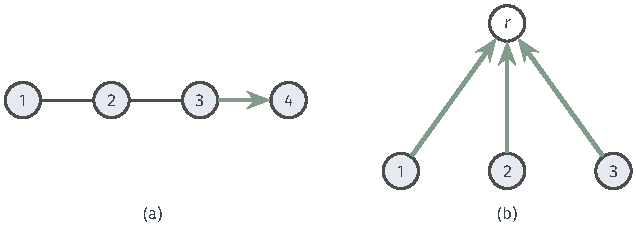
\includegraphics[width=107.500mm]{figures/03-graphs/04-local-functions-and-dynamic-programming/tikz/dp-message-frontier/figure.pdf}
  \caption{同时存活的消息决定峰值存储。圆点表示袋，绿色箭头表示已经生成、仍待父袋读取的消息。(a)链上袋$1,2$的消息已被后继使用并释放，仅袋$3$的消息仍在；(b)根$r$尚未处理，三个叶袋的消息同时存在。此处比较消息存储，不包含回溯表或输出表。}
  \label{fig:graph-dp-message-frontier}
\end{figure}

需要恢复配置时，回溯表要保留到前序回溯走完，存储为$\sum_u|\mathcal X_{S_u}|\cdot|I_u|$量级，这时可以释放的只有消息。

四环算例中，最小成本计算的峰值是一条$4$项消息加根处的工作空间；恢复配置还要保留一张$4$项的回溯表。$R=\{1,3\}$的查询中，处理根之前两条$4$项消息同时存在，输出表另有$4$项。

\subsection{时间与存储的取舍}
\label{sec:graph-dp-time-memory-tradeoff}

固定同一结构和输出要求，可以在三种做法之间取舍：缓存中间结果、在最后一次使用后释放、或者按需重算。

最直接的是全部缓存：保留所有消息和回溯表，向上一遍后既能恢复配置，也能再发一遍反向消息得到每个袋的表，时间最少，存储最多。只需最优值时，在最后一次使用后立即释放消息，存储降到上一小节的峰值，时间不变。

回溯表也可以不存。若保留各条子消息，恢复时对每个节点$u$在已知接口取值下重新枚举$\bm x_{I_u}$、重算$g_u$并取最小点，就能得到与回溯表相同的选择（并列规则保持一致即可）；额外时间是每个节点$|\mathcal X_{I_u}|$量级的重算，存储从回溯表换成消息。若连消息也释放了，恢复时就要重新计算子树的消息，时间可能成倍增加。总之，释放后仍要用到的信息只能重算，或者从另存的记录中读回。

是否恢复配置、是否保存整张保留变量表，都会改变记录的保留时机。只要整体最优值时，回溯表根本不必生成；只要条件最小成本表而不要条件最优配置时，根处的回溯表可以省去。

只查询少数几个$\bm x_R$而不是整张表时，可以对每个查询值把$\bm x_R$固定后按第~\ref{sec:graph-dp-min-cost}节计算一次，用查询次数乘以单次时间换取不必存放$|\mathcal X_R|$项的输出表。哪种做法更合适，取决于结构的实际规模和输出要求，应在固定任务后按上面的资源指标比较。
